% Who has the ball? -- problem, data, baseline and our solution.
% Build:  cd slides && latexmk -pdf main.tex      (figure data: python slides/make_data.py)
\documentclass[aspectratio=169,10pt]{beamer}

\usetheme[progressbar=frametitle,numbering=fraction,block=fill,sectionpage=none]{metropolis}
\usepackage[sfdefault,lining]{FiraSans}
\usepackage{FiraMono}
\usepackage[T1]{fontenc}
\usepackage{amsmath,amssymb}
\usepackage{booktabs}
\usepackage{tikz}
\usepackage{pgfplots}
\pgfplotsset{compat=1.18}
\usetikzlibrary{arrows.meta,positioning,calc,decorations.pathreplacing,shapes.misc}

% -- colours ----------------------------------------------------------------------------------
\definecolor{cH}{HTML}{1F5FA8}      % home, Barcelona
\definecolor{cA}{HTML}{D1342F}      % away, Athletic
\definecolor{cD}{HTML}{A6A6A6}      % dead ball
\definecolor{cX}{HTML}{EEEEEE}
\definecolor{accent}{HTML}{E08A1E}
\definecolor{ink}{HTML}{23373B}
\definecolor{soft}{HTML}{F2F4F5}
\definecolor{good}{HTML}{2E8B57}
\setbeamercolor{alerted text}{fg=accent}

\newcommand{\Hl}{\textcolor{cH}{\textbf{H}}}
\newcommand{\Al}{\textcolor{cA}{\textbf{A}}}
\newcommand{\Dl}{\textcolor{cD!80!black}{\textbf{D}}}
\newcommand{\Xl}{\textcolor{black!50}{\textbf{X}}}
\newcommand{\takeaway}[1]{%
  \vfill
  \begin{tikzpicture}
    \node[fill=accent!12,draw=accent,rounded corners=2pt,inner sep=5pt,text width=0.94\textwidth,
          align=center,font=\small]{#1};
  \end{tikzpicture}}

% -- timeline strips: \seg{start s}{end s}{H|A|D} inside a strip ----------------------------------
\newcommand{\sx}{0.041}   % cm per second of match
\newcommand{\hh}{0.42}    % strip height, cm
\def\yy{0}
\newcommand{\seg}[3]{\fill[c#3] ({#1*\sx},{\yy}) rectangle ({#2*\sx},{\yy+\hh});}
\newcommand{\strip}[3]{% y, label, file
  \def\yy{#1}
  \node[anchor=east,font=\scriptsize] at (-0.1,{#1+\hh/2}) {#2};
  \input{#3}
  \draw[black!40,line width=0.2pt] (0,#1) rectangle ({300*\sx},{#1+\hh});}
\newcommand{\timeaxis}[1]{% y
  \draw[black!50] (0,#1) -- ({300*\sx},#1);
  \foreach \m in {0,1,...,5} {
    \draw[black!50] ({60*\m*\sx},#1) -- ({60*\m*\sx},{#1-0.08});
    \node[font=\tiny,below] at ({60*\m*\sx},{#1-0.05}) {\m:00};}}
\newcommand{\stripkey}{%
  {\scriptsize\textcolor{cH}{$\blacksquare$}~home (Barça) \quad
   \textcolor{cA}{$\blacksquare$}~away (Athletic) \quad
   \textcolor{cD}{$\blacksquare$}~dead ball}}

% -- pitch, drawn in metres (105 x 68) ---------------------------------------------------------
\newcommand{\pitchbg}{\fill[green!8] (-2,-2) rectangle (107,70);}
\newcommand{\pitchlines}{%
  \draw[black!45,line width=0.4pt]
    (0,0) rectangle (105,68)  (52.5,0) -- (52.5,68)  (52.5,34) circle (9.15)
    (0,13.84) rectangle (16.5,54.16)  (105,13.84) rectangle (88.5,54.16)
    (0,24.84) rectangle (5.5,43.16)   (105,24.84) rectangle (99.5,43.16)
    (0,30.34) rectangle (-1.5,37.66)  (105,30.34) rectangle (106.5,37.66);
  \fill[black!45] (52.5,34) circle (0.5);}

\pgfplotsset{
  slide/.style={
    width=7.4cm, height=4.6cm, axis lines=left, tick align=outside,
    tick label style={font=\scriptsize}, label style={font=\scriptsize},
    legend style={font=\scriptsize,draw=none,fill=none}, every axis plot/.append style={line width=0.9pt},
    enlarge x limits=0.02, ymajorgrids, grid style={black!10}},
}

\title{Who has the ball?}
\subtitle{Frame-level ball possession from automatic tracking data\\[2pt]
  \small More than a Hack 2027 · Phase 1}
\author{} % team names
\date{\today}

\begin{document}

\maketitle

% ================================================================================================
\section{The problem}
% ================================================================================================

\begin{frame}{The task: for every frame, who has the ball?}
  \centering
  \begin{tikzpicture}
    \strip{0}{5 min of truth}{data/strip_gt.tex}
    \timeaxis{-0.05}
  \end{tikzpicture}

  \stripkey

  \vspace{0.4cm}
  \begin{columns}[T]
    \begin{column}{0.45\textwidth}
      \textbf{Input / output}
      \begin{itemize}\small
        \item 1 full match: Barça (\Hl) vs Athletic (\Al)
        \item 199{,}319 frames at 25 fps; 158{,}857 graded (the two halves)
        \item one label per frame: \Hl\ / \Al\ / \Dl\ (or \Xl\ = no answer)
      \end{itemize}
    \end{column}
    \begin{column}{0.5\textwidth}
      \textbf{Possession rules}
      \begin{itemize}\small
        \item changes only when the other team gets \alert{control}
        \item loose or contested ball $\to$ stays with the last team
        \item a touch, deflection or aerial duel without control is not a change
        \item ball out of play $\to$ \Dl, never a possession
      \end{itemize}
    \end{column}
  \end{columns}
\end{frame}

\begin{frame}{How we are scored: whole possessions, not frames}
  \begin{columns}[c]
    \begin{column}{0.48\textwidth}
      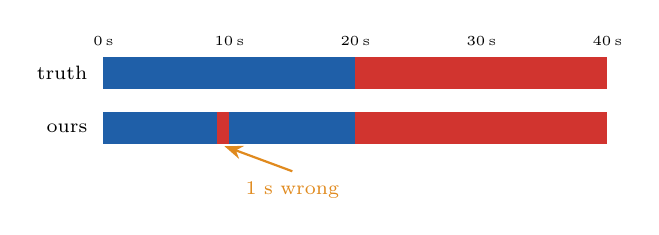
\begin{tikzpicture}[x=0.16cm,y=1cm]
        \foreach \t in {0,10,20,30,40} \node[font=\tiny] at (\t,1.6) {\t\,s};
        \node[anchor=east,font=\scriptsize] at (-0.5,1.2) {truth};
        \fill[cH] (0,1) rectangle (20,1.4); \fill[cA] (20,1) rectangle (40,1.4);
        \node[anchor=east,font=\scriptsize] at (-0.5,0.5) {ours};
        \fill[cH] (0,0.3) rectangle (9,0.7); \fill[cA] (9,0.3) rectangle (10,0.7);
        \fill[cH] (10,0.3) rectangle (20,0.7); \fill[cA] (20,0.3) rectangle (40,0.7);
        \draw[accent,thick,-{Stealth}] (15,-0.05) node[below,font=\scriptsize,text=accent]
          {1 s wrong} -- (9.6,0.27);
      \end{tikzpicture}

      \vspace{0.3cm}
      \begin{tabular}{lr}
        \toprule
        frame accuracy & 97.5\% \\
        \textbf{spellF1} & \textbf{0.53} \\
        \bottomrule
      \end{tabular}
    \end{column}
    \begin{column}{0.48\textwidth}
      \textbf{spellF1} (ranking)
      \begin{itemize}\small
        \item each possession (run of \Hl\ or \Al) is one object
        \item matched 1-to-1 to the truth by time overlap (IoU)
        \item F1 averaged over IoU thresholds 0.3 -- 0.7
        \item 1 frame late: free · 1 s late: 0.65
      \end{itemize}
      \vspace{0.1cm}
      \textbf{macroF1} (tie-break)
      \begin{itemize}\small
        \item per-frame F1 of \Hl, \Al, \Dl, averaged
      \end{itemize}
    \end{column}
  \end{columns}
  \takeaway{Splitting or inventing possessions is what costs points. We only get
    \textbf{5 minutes (17 possessions)} of labels, too few to tune on.}
\end{frame}

% ================================================================================================
\section{The data}
% ================================================================================================

\begin{frame}{What we have}
  \begin{columns}[c]
    \begin{column}{0.55\textwidth}
      \centering\small
      \begin{tabular}{lll}
        \toprule
        & \textbf{tactical cam} & \textbf{broadcast cam} \\
        \midrule
        video & 199{,}319 frames & own timeline, replays \\
        tracking & players + ball & players + ball \\
        ball tracked & 57\% & 51\% \\
        homography & 100\% & 66\% \\
        Smart Tagging & 638 tags & --- \\
        \bottomrule
      \end{tabular}
    \end{column}
    \begin{column}{0.42\textwidth}
      \begin{itemize}\small
        \item all \textbf{automatic}, not corrected by hand
        \item \textbf{no player IDs}: 46 track slots for 22 players, only the team is known
        \item tracker swaps the two goalkeepers
        \item broadcast is \textbf{not synchronised} with tactical
        \item Smart Tagging: phases and set pieces, also automatic
      \end{itemize}
    \end{column}
  \end{columns}
  \takeaway{We use only the tracking of both cameras. Smart Tagging is kept as an independent check.}
\end{frame}

% ================================================================================================
\section{Exploratory analysis}
% ================================================================================================

\begin{frame}{EDA: the ball is missing on 41\% of frames}
  \begin{columns}[c]
    \begin{column}{0.55\textwidth}
      \centering
      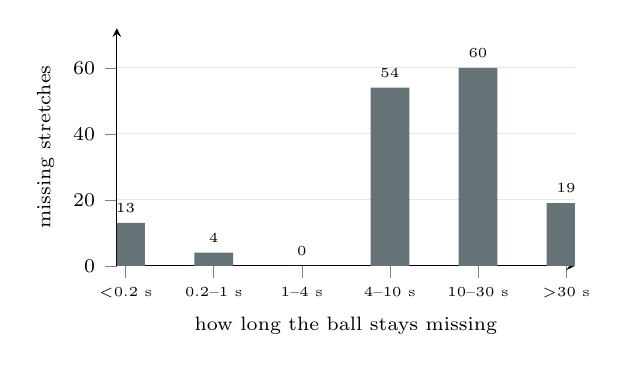
\begin{tikzpicture}
        \begin{axis}[slide, ybar, bar width=14pt, ymin=0, ymax=72,
            xtick={0,...,5}, xticklabels={$<$0.2 s, 0.2--1 s, 1--4 s, 4--10 s, 10--30 s, $>$30 s},
            x tick label style={font=\tiny}, ylabel={missing stretches},
            xlabel={how long the ball stays missing},
            nodes near coords, every node near coord/.append style={font=\tiny}]
          \addplot[fill=ink!70,draw=none] coordinates {(0,13) (1,4) (2,0) (3,54) (4,60) (5,19)};
        \end{axis}
      \end{tikzpicture}
    \end{column}
    \begin{column}{0.42\textwidth}
      \begin{itemize}\small
        \item median missing stretch: \textbf{10.7 s}
        \item no gaps of 1--4 s: the tracker \textbf{interpolates} them, so a ``tracked'' ball can be in
              the wrong place
      \end{itemize}
      \vspace{0.1cm}
      \centering\small
      \begin{tabular}{lr}
        \toprule
        & ball missing \\
        \midrule
        ball in play & 6.5\% \\
        dead ball & \textbf{33.6\%} \\
        \bottomrule
      \end{tabular}
    \end{column}
  \end{columns}
  \takeaway{Gone for seconds, not frames. A missing ball is \textbf{5$\times$ likelier} when play is
    stopped.}
\end{frame}

\begin{frame}{EDA: players walk when the ball is dead}
  \begin{columns}[c]
    \begin{column}{0.58\textwidth}
      \centering
      \begin{tikzpicture}
        \begin{axis}[slide, width=8cm, height=5.1cm, xmin=0, xmax=7, ymin=0,
            xlabel={speed of the 5 fastest players, 1 s average (m/s)},
            ylabel={share of frames}, yticklabel style={/pgf/number format/fixed},
            legend pos=north east, scaled y ticks=false]
          \addplot[cD!70!black, fill=cD!30, fill opacity=0.6] table[x=x,y=dead] {data/activity.dat}
            \closedcycle;
          \addplot[cH, fill=cH!20, fill opacity=0.5] table[x=x,y=live] {data/activity.dat}
            \closedcycle;
          \draw[accent, thick] (axis cs:2.6,0) -- (axis cs:2.6,0.22);
          \node[accent, font=\scriptsize, anchor=west] at (axis cs:2.65,0.2) {2.6 m/s};
          \legend{dead ball, ball in play}
        \end{axis}
      \end{tikzpicture}
    \end{column}
    \begin{column}{0.39\textwidth}
      \begin{itemize}\small
        \item median in play: \textbf{3.9 m/s}
        \item median in a stoppage: \textbf{1.9 m/s}
        \item the full-match histogram has a valley at \textbf{2.6 m/s}: our threshold, found
              without labels
        \item limit: slow build-up at the back also looks like walking
      \end{itemize}
    \end{column}
  \end{columns}
  \takeaway{Player movement tells us \textbf{if the ball is in play}, even when the ball is not tracked.}
\end{frame}

\begin{frame}{EDA: ``nearest player'' is a weak signal}
  \begin{columns}[c]
    \begin{column}{0.5\textwidth}
      \centering
      \begin{tikzpicture}
        \begin{axis}[slide, ybar, bar width=6pt, xmin=0, xmax=10, ymin=0,
            xlabel={ball to nearest player (m), ball in play},
            ylabel={share of frames}, yticklabel style={/pgf/number format/fixed},
            scaled y ticks=false]
          \addplot[fill=ink!65,draw=none] table[x=x,y=share] {data/dist.dat};
          \fill[accent, opacity=0.15] (axis cs:0,0) rectangle (axis cs:1.5,0.21);
          \node[accent, font=\scriptsize, anchor=west] at (axis cs:1.6,0.19) {1.5 m};
        \end{axis}
      \end{tikzpicture}
    \end{column}
    \begin{column}{0.47\textwidth}
      \centering\small
      \begin{tabular}{lrr}
        \toprule
        signal & right team & frames \\
        \midrule
        nearest player & 79\% & 94\% \\
        \textbf{clear contact} & \textbf{92\%} & 41\% \\
        \bottomrule
      \end{tabular}

      \vspace{0.3cm}
      \raggedright
      \textbf{clear contact} = ball within 1.5 m of a player of \emph{exactly one} team
      \begin{itemize}\small
        \item duel or ball in flight $\to$ no evidence
        \item 1.5 m = touching distance + $\approx$0.5 m tracking noise
      \end{itemize}
    \end{column}
  \end{columns}
  \takeaway{Fewer but reliable observations beat a noisy guess on every frame.}
\end{frame}

\begin{frame}{EDA: the 5 labelled minutes}
  \centering
  \begin{tikzpicture}
    \strip{0}{truth}{data/strip_gt.tex}
    \timeaxis{-0.05}
  \end{tikzpicture}

  \stripkey

  \vspace{0.4cm}
  \begin{columns}[T]
    \begin{column}{0.3\textwidth}
      \centering
      {\Large\textbf{17}}\\ possessions, 4 stoppages\\
      \small Barça 57\% · dead ball 20\%
    \end{column}
    \begin{column}{0.3\textwidth}
      \centering
      {\Large\textbf{0.8 -- 42 s}}\\ median 7.6 s\\
      \small 6 of 17 shorter than 4 s
    \end{column}
    \begin{column}{0.3\textwidth}
      \centering
      {\Large\textbf{+0.8 s}}\\ label changes after the new team's first touch\\
      \small (restarts: +0.4 s after the kick)
    \end{column}
  \end{columns}
  \takeaway{Long possessions are easy. The \textbf{short ones} and the exact change times decide
    the score.}
\end{frame}

% ================================================================================================
\section{Baseline}
% ================================================================================================

\begin{frame}{Baseline: nearest player + majority vote}
  \begin{columns}[T]
    \begin{column}{0.42\textwidth}
      \centering
      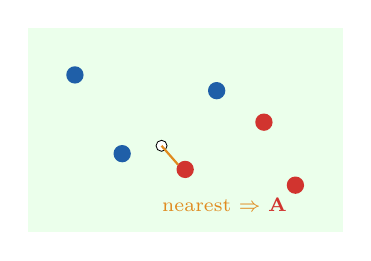
\begin{tikzpicture}[scale=0.1]
        \fill[green!8] (0,0) rectangle (40,26);
        \fill[cH] (12,10) circle (1.1); \fill[cH] (24,18) circle (1.1); \fill[cH] (6,20) circle (1.1);
        \fill[cA] (20,8) circle (1.1); \fill[cA] (30,14) circle (1.1); \fill[cA] (34,6) circle (1.1);
        \fill[white,draw=black,line width=0.3pt] (17,11) circle (0.7);
        \draw[accent,thick] (17,11) -- (19.1,8.6);
        \node[font=\scriptsize,accent] at (25,3.5) {nearest $\Rightarrow$ \Al};
      \end{tikzpicture}

      \vspace{0.2cm}
      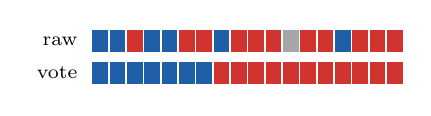
\begin{tikzpicture}[x=0.22cm,y=0.4cm]
        \node[font=\scriptsize,anchor=east] at (-0.3,1.5) {raw};
        \foreach \i/\c in {0/H,1/H,2/A,3/H,4/H,5/A,6/A,7/H,8/A,9/A,10/A,11/D,12/A,13/A,14/H,15/A,16/A,17/A}
          \fill[c\c] (\i,1.15) rectangle (\i+0.9,1.85);
        \node[font=\scriptsize,anchor=east] at (-0.3,0.5) {vote};
        \foreach \i/\c in {0/H,1/H,2/H,3/H,4/H,5/H,6/H,7/A,8/A,9/A,10/A,11/A,12/A,13/A,14/A,15/A,16/A,17/A}
          \fill[c\c] (\i,0.15) rectangle (\i+0.9,0.85);
      \end{tikzpicture}

      \vspace{0.2cm}
      \raggedright
      \begin{enumerate}\small
        \item ball tracked $\to$ team of the nearest player; else \Dl
        \item majority vote over a $\pm w$ window
      \end{enumerate}
    \end{column}
    \begin{column}{0.55\textwidth}
      \centering
      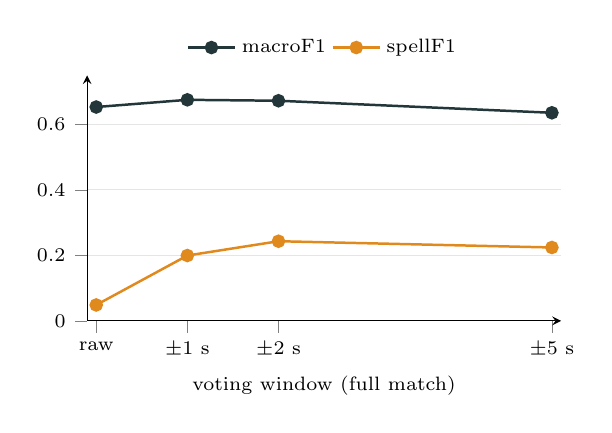
\begin{tikzpicture}
        \begin{axis}[slide, width=7.6cm, height=4.7cm,
            xtick={0,25,50,125}, xticklabels={raw,$\pm$1 s,$\pm$2 s,$\pm$5 s},
            xlabel={voting window (full match)},
            ymin=0, ymax=0.75, legend columns=2,
            legend style={at={(0.5,1.03)},anchor=south}]
          \addplot[mark=*, ink] coordinates {(0,0.6532) (25,0.6752) (50,0.6724) (125,0.6356)};
          \addplot[mark=*, accent] coordinates {(0,0.0486) (25,0.1996) (50,0.2433) (125,0.2242)};
          \legend{macroF1, spellF1}
        \end{axis}
      \end{tikzpicture}

      \raggedright
      \begin{itemize}\small
        \item one parameter: macroF1 moves 0.04, spellF1 $\times$5
        \item public 5 min prefer $\pm$5 s; the full match prefers $\pm$2 s
        \item \textbf{floor to beat: spellF1 0.243}
      \end{itemize}
    \end{column}
  \end{columns}
\end{frame}

\begin{frame}{Baseline: what goes wrong}
  \centering
  \begin{tikzpicture}
    \strip{1.4}{truth}{data/strip_gt.tex}
    \strip{0.7}{vote $\pm$2 s}{data/strip_b50.tex}
    \strip{0}{raw}{data/strip_raw.tex}
    \timeaxis{-0.05}
  \end{tikzpicture}

  \stripkey

  \vspace{0.4cm}
  \begin{columns}[T]
    \begin{column}{0.3\textwidth}
      \centering
      \textbf{flicker}\\ \small 131 (raw) and 26 ($\pm$2 s) possessions vs 17 true;
      smoothing makes changes late
    \end{column}
    \begin{column}{0.3\textwidth}
      \centering
      \textbf{\Dl\ = ball not seen}\\ \small stoppages found by accident: \Dl\ F1 only 0.15 -- 0.42
    \end{column}
    \begin{column}{0.3\textwidth}
      \centering
      \textbf{no restart logic}\\ \small the restarting team is whoever stands nearest
    \end{column}
  \end{columns}
\end{frame}

% ================================================================================================
\section{Our solution}
% ================================================================================================

\begin{frame}{Our solution: overview}
  \centering
  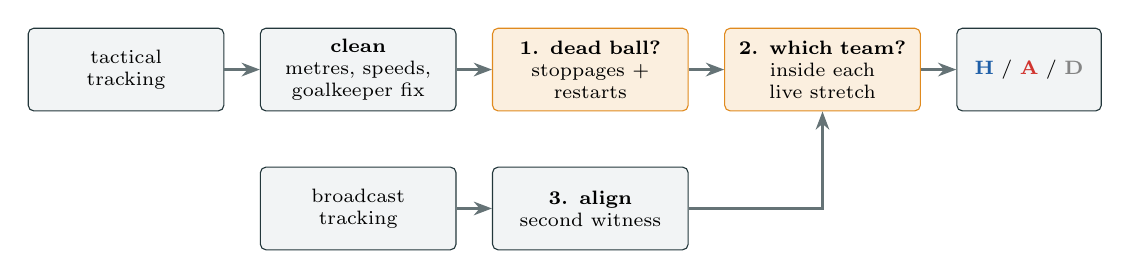
\begin{tikzpicture}[
      box/.style={draw=ink,rounded corners=2pt,fill=soft,align=center,font=\scriptsize,
                  minimum height=1.05cm,text width=2.25cm},
      key/.style={box,fill=accent!14,draw=accent},
      arr/.style={-{Stealth},thick,ink!70}, node distance=0.45cm]
    \node[box] (atd) {tactical\\tracking};
    \node[box,right=of atd] (load) {\textbf{clean}\\metres, speeds,\\goalkeeper fix};
    \node[key,right=of load] (dead) {\textbf{1. dead ball?}\\stoppages +\\restarts};
    \node[key,right=of dead] (poss) {\textbf{2. which team?}\\inside each\\live stretch};
    \node[box,right=of poss,text width=1.6cm] (csv) {\Hl\ / \Al\ / \Dl};
    \node[box,below=0.7cm of load] (bc) {broadcast\\tracking};
    \node[box,right=of bc] (align) {\textbf{3. align}\\second witness};
    \draw[arr] (atd) -- (load); \draw[arr] (load) -- (dead); \draw[arr] (dead) -- (poss);
    \draw[arr] (poss) -- (csv); \draw[arr] (bc) -- (align); \draw[arr] (align) -| (poss);
  \end{tikzpicture}

  \vspace{0.5cm}
  \begin{columns}[T]
    \begin{column}{0.3\textwidth}\centering
      \textbf{tracking only}\\ \small no video pixels, no Smart Tagging, no labels
    \end{column}
    \begin{column}{0.3\textwidth}\centering
      \textbf{one tool, used twice}\\ \small the same two-state decoder for dead/alive and home/away
    \end{column}
    \begin{column}{0.3\textwidth}\centering
      \textbf{no tuning on the 5 min}\\ \small numbers from physics, the Laws of the Game, or the
      unlabelled full match
    \end{column}
  \end{columns}

  \vspace{0.3cm}
  \scriptsize Goalkeeper fix: a keeper track gets the team that defends the half it is in.
  Pure numpy, deterministic.
\end{frame}

\begin{frame}{The core tool: a two-state decoder}
  Each frame gets a cost $c_t(s)$ for each answer $s\in\{0,1\}$. We pick the labelling that minimises
  \[
    \underbrace{\sum_{t} c_t(s_t)}_{\text{disagreement with the evidence}}
    \;+\; \lambda\cdot\underbrace{\sum_{t} \mathbf{1}[s_t\ne s_{t-1}]}_{\text{number of changes}}
  \]
  \vspace{-0.2cm}
  \begin{columns}[c]
    \begin{column}{0.44\textwidth}
      \begin{itemize}\small
        \item solved exactly in $O(T)$ by dynamic programming (Viterbi):\\[2pt]
              \mbox{\scriptsize $A_t(s) = c_t(s) + \min\{A_{t-1}(s),\, A_{t-1}(1{-}s)+\lambda\}$}
        \item the state changes only if the evidence against it adds up to more than $\lambda$
        \item no evidence $\to$ the state is kept
      \end{itemize}
    \end{column}
    \begin{column}{0.53\textwidth}
      \centering
      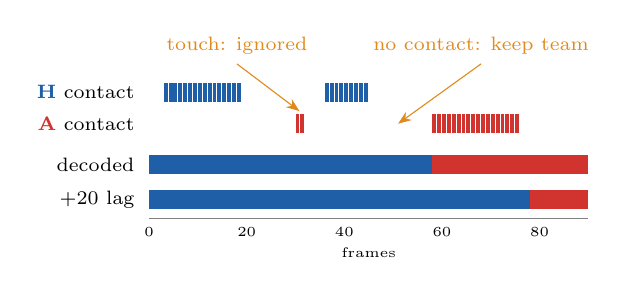
\begin{tikzpicture}[x=0.062cm,y=0.8cm]
        \node[font=\scriptsize,anchor=east] at (-1,1.85) {\Hl\ contact};
        \node[font=\scriptsize,anchor=east] at (-1,1.35) {\Al\ contact};
        \foreach \t in {3,...,18,36,37,...,44} \fill[cH] (\t,1.7) rectangle (\t+0.8,2.0);
        \foreach \t in {30,31} \fill[cA] (\t,1.2) rectangle (\t+0.8,1.5);
        \foreach \t in {58,...,75} \fill[cA] (\t,1.2) rectangle (\t+0.8,1.5);
        \node[font=\scriptsize,anchor=east] at (-1,0.7) {decoded};
        \fill[cH] (0,0.55) rectangle (58,0.85); \fill[cA] (58,0.55) rectangle (90,0.85);
        \node[font=\scriptsize,anchor=east] at (-1,0.15) {+20 lag};
        \fill[cH] (0,0) rectangle (78,0.3); \fill[cA] (78,0) rectangle (90,0.3);
        \draw[accent,-{Stealth}] (18,2.3) node[above,font=\scriptsize,text=accent]
          {touch: ignored} -- (30.8,1.55);
        \draw[accent,-{Stealth}] (68,2.3) node[above,font=\scriptsize,text=accent]
          {no contact: keep team} -- (51,1.35);
        \draw[black!50] (0,-0.15) -- (90,-0.15);
        \foreach \t in {0,20,...,80} \node[font=\tiny,below] at (\t,-0.15) {\t};
        \node[font=\tiny] at (45,-0.7) {frames};
      \end{tikzpicture}
    \end{column}
  \end{columns}
  \takeaway{Flickering per-frame evidence $\to$ \textbf{whole stoppages and whole possessions}.}
\end{frame}

\begin{frame}{Step 1: dead ball}
  \begin{columns}[T]
    \begin{column}{0.5\textwidth}
      \textbf{1. Score} each frame (log-odds of ``dead'')
      \vspace{0.05cm}

      \small
      \begin{tabular}{lr}
        \toprule
        players walking ($<$2.6 m/s) & up to $+4$ \\
        ball not tracked & $+1.5$ \\
        ball beyond a line & $+4$ \\
        fewer than 18 players tracked & $+1$ \\
        \bottomrule
      \end{tabular}

      \vspace{0.15cm}
      \normalsize\textbf{2. Decode}: $\lambda=40$ ($\approx$ 2 s of evidence to open or close a stoppage)

      \vspace{0.1cm}
      \textbf{3. Restart}: ball goes from quiet to played ($\ge$5 m/s);
      the stoppage ends 10 frames later

      \vspace{0.1cm}
      \textbf{4. Tidy}: drop stoppages $<$2 s, and $<$6 s ones with no line crossed and no restart
    \end{column}
    \begin{column}{0.47\textwidth}
      \centering
      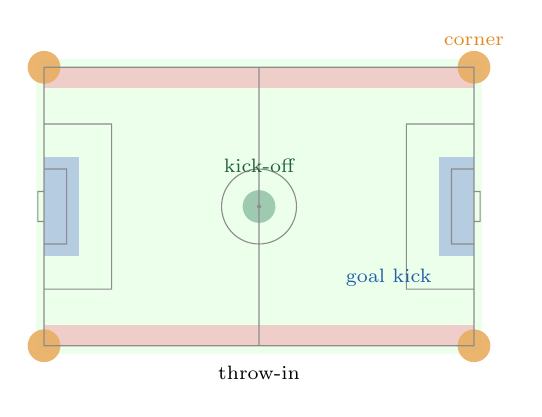
\begin{tikzpicture}[scale=0.052]
        \pitchbg
        \fill[cA!30,opacity=0.8] (0,0) rectangle (105,5);
        \fill[cA!30,opacity=0.8] (0,63) rectangle (105,68);
        \fill[cH!35,opacity=0.9] (0,21.84) rectangle (8.5,46.16);
        \fill[cH!35,opacity=0.9] (105,21.84) rectangle (96.5,46.16);
        \foreach \x/\y in {0/0,105/0,0/68,105/68} \fill[accent!70,opacity=0.9] (\x,\y) circle (4);
        \fill[good!50,opacity=0.9] (52.5,34) circle (4);
        \pitchlines
        \node[font=\scriptsize,anchor=north] at (52.5,-2.5) {throw-in};
        \node[font=\scriptsize,anchor=north east,cH] at (97,21) {goal kick};
        \node[font=\scriptsize,anchor=south,accent] at (105,71) {corner};
        \node[font=\scriptsize,anchor=south,good!70!black] at (52.5,40) {kick-off};
      \end{tikzpicture}

      \vspace{0.2cm}
      \raggedright\small
      \textbf{Latch}: ball out $\to$ dead until a restart from a spot the Laws allow
      \begin{itemize}\scriptsize
        \item goal line $\to$ corner, goal kick, or kick-off after a goal
        \item touchline $\to$ throw-in
      \end{itemize}
    \end{column}
  \end{columns}
\end{frame}

\begin{frame}{Step 2: which team}
  \centering
  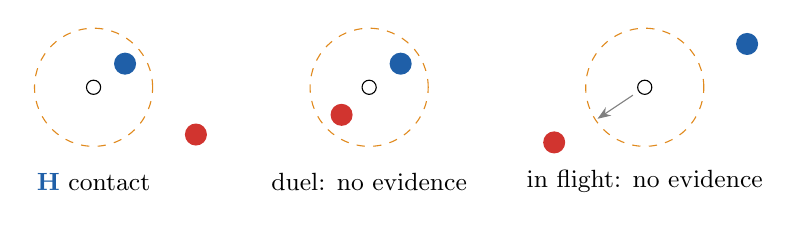
\begin{tikzpicture}[scale=0.5]
    \begin{scope}
      \draw[accent,dashed] (0,0) circle (1.5);
      \fill[white,draw=black] (0,0) circle (0.18);
      \fill[cH] (0.8,0.6) circle (0.28); \fill[cA] (2.6,-1.2) circle (0.28);
      \node[font=\small] at (0,-2.4) {\Hl\ contact};
    \end{scope}
    \begin{scope}[xshift=7cm]
      \draw[accent,dashed] (0,0) circle (1.5);
      \fill[white,draw=black] (0,0) circle (0.18);
      \fill[cH] (0.8,0.6) circle (0.28); \fill[cA] (-0.7,-0.7) circle (0.28);
      \node[font=\small] at (0,-2.4) {duel: no evidence};
    \end{scope}
    \begin{scope}[xshift=14cm]
      \draw[accent,dashed] (0,0) circle (1.5);
      \fill[white,draw=black] (0,0) circle (0.18);
      \fill[cH] (2.6,1.1) circle (0.28); \fill[cA] (-2.3,-1.4) circle (0.28);
      \draw[black!50,-{Stealth}] (-0.3,-0.2) -- (-1.2,-0.8);
      \node[font=\small] at (0,-2.4) {in flight: no evidence};
    \end{scope}
  \end{tikzpicture}

  \vspace{0.3cm}
  \begin{columns}[T]
    \begin{column}{0.31\textwidth}
      \textbf{Decoder, $\lambda=8$}
      \begin{itemize}\footnotesize
        \item cost of saying \Hl\ = 1 per frame of \Al\ contact
        \item a change needs $>$8 frames of the other team's contact
        \item single touches and deflections never flip the team
      \end{itemize}
    \end{column}
    \begin{column}{0.31\textwidth}
      \textbf{Timing: +20 frames}
      \begin{itemize}\footnotesize
        \item the truth changes at \emph{control}, not at the first touch
        \item 20 = median gap measured on the 5 public minutes
      \end{itemize}
    \end{column}
    \begin{column}{0.31\textwidth}
      \textbf{Who restarts play}
      \begin{itemize}\footnotesize
        \item corner $\to$ attacking team
        \item goal kick $\to$ defending team
        \item else the team standing at the ball
        \item else the team that did not touch it last
      \end{itemize}
    \end{column}
  \end{columns}
\end{frame}

\begin{frame}{Step 3: the broadcast camera as a second witness}
  \centering
  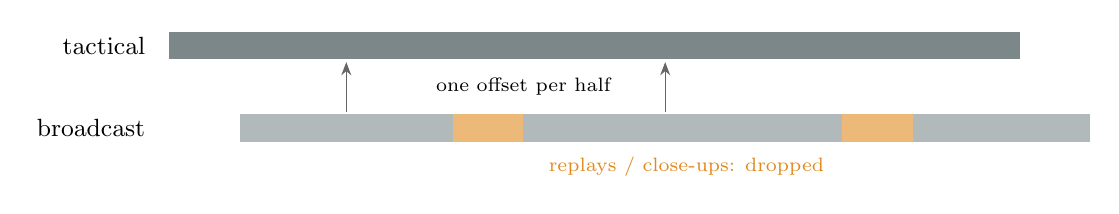
\begin{tikzpicture}[x=0.9cm,y=0.7cm,font=\small]
    \node[anchor=east] at (-0.2,2.25) {tactical};
    \fill[ink!60] (0,2) rectangle (12,2.5);
    \node[anchor=east] at (-0.2,0.75) {broadcast};
    \fill[ink!35] (1,0.5) rectangle (4,1); \fill[accent!60] (4,0.5) rectangle (5,1);
    \fill[ink!35] (5,0.5) rectangle (9.5,1); \fill[accent!60] (9.5,0.5) rectangle (10.5,1);
    \fill[ink!35] (10.5,0.5) rectangle (13,1);
    \draw[-{Stealth},black!60] (2.5,1.05) -- (2.5,1.95);
    \draw[-{Stealth},black!60] (7,1.05) -- (7,1.95);
    \node[accent,font=\scriptsize] at (7.3,0.05) {replays / close-ups: dropped};
    \node[font=\scriptsize] at (5,1.5) {one offset per half};
  \end{tikzpicture}

  \vspace{0.4cm}
  \begin{columns}[T]
    \begin{column}{0.31\textwidth}
      \textbf{1. Align}
      \begin{itemize}\footnotesize
        \item live TV runs in real time: one constant offset per half
        \item found by matching the two ball tracks: 4{,}014 and 26{,}920 frames
      \end{itemize}
    \end{column}
    \begin{column}{0.31\textwidth}
      \textbf{2. Gate}
      \begin{itemize}\footnotesize
        \item keep a frame only if its players stand where the tactical players are
              (median gap $\le$1.5 m, $\ge$6 players)
      \end{itemize}
    \end{column}
    \begin{column}{0.31\textwidth}
      \textbf{3. Fill gaps}
      \begin{itemize}\footnotesize
        \item same clear-contact rule
        \item counts 0.72 of a tactical frame, only where tactical sees no contact
      \end{itemize}
    \end{column}
  \end{columns}
  \takeaway{Zoomed in on the ball, the broadcast camera sees duels the wide camera blurs.}
\end{frame}

% ================================================================================================
\section{Results}
% ================================================================================================

\begin{frame}{Results on the public 5 minutes}
  \begin{columns}[c]
    \begin{column}{0.6\textwidth}
      \centering\small
      \begin{tabular}{lccc}
        \toprule
        & spellF1 & macroF1 & possessions \\
        \midrule
        truth & --- & --- & 17 \\
        baseline $\pm$2 s & 0.326 & 0.621 & 26 \\
        ours, tactical & 0.520 & 0.913 & 13 \\
        \textbf{ours + broadcast} & \textbf{0.581} & \textbf{0.926} & 14 \\
        \bottomrule
      \end{tabular}
    \end{column}
    \begin{column}{0.37\textwidth}
      \begin{itemize}\footnotesize
        \item dead-ball F1 \textbf{0.96} (baseline 0.15 -- 0.42)
        \item all 4 stoppages found
        \item 17 possessions only: spellF1 band 0.39 -- 0.76
      \end{itemize}
    \end{column}
  \end{columns}

  \vspace{0.3cm}
  \centering
  \begin{tikzpicture}
    \strip{1.4}{truth}{data/strip_gt.tex}
    \strip{0.7}{ours}{data/strip_sol.tex}
    \strip{0}{baseline}{data/strip_b50.tex}
    \timeaxis{-0.05}
  \end{tikzpicture}
  \takeaway{Per frame almost solved (0.93). Per possession not yet (0.58): we miss the
    \textbf{short} ones.}
\end{frame}

\begin{frame}{Full match and what is left}
  \begin{columns}[T]
    \begin{column}{0.44\textwidth}
      \textbf{Full match} (no labels needed)
      \vspace{0.1cm}

      \small
      \begin{tabular}{lr}
        \toprule
        dead ball (real matches: 40 -- 50\%) & 49\% \\
        possessions (mean 10.7 s) & 303 \\
        Smart Tagging restarts we find & 92\% \\
        restart team agrees with the tag & 79\% \\
        \bottomrule
      \end{tabular}

      \vspace{0.2cm}
      \scriptsize Every parameter halved and doubled: most results stay within the noise.
    \end{column}
    \begin{column}{0.52\textwidth}
      \textbf{Our 9 errors}, checked on video
      \vspace{0.1cm}

      \small
      \begin{tabular}{lr}
        \toprule
        tracker ball in the wrong place & 3 \\
        touch without control counted & 2 \\
        missed very short tackle / duel & 2 \\
        stoppage, ball still rolling & 1 \\
        tie (whistle not visible) & 1 \\
        \bottomrule
      \end{tabular}

      \vspace{0.2cm}
      \scriptsize Tried, no gain: lower switch costs, duel evidence, team-shape classifier.
    \end{column}
  \end{columns}
  \takeaway{With perfect stoppages put in by hand the score does not move:
    the loss is \textbf{in-play changes} the tracking barely shows.}
\end{frame}

\begin{frame}[standout]
  Questions?
\end{frame}

\end{document}
